\chapter{Data Analysis}

In this section we explore the given data and draw some preliminary observations which help us to build our models. We discuss any shortcomings and show why we have opted for certain pre-processing techniques. The pre-processing techniques and a how they were conducted are then discussed.

\section{Preliminary Data Exploration}

We are provided with 2 datasets. The training dataset contains 458 days, half of which are NPF events and half are not. The distribution of classes is displayed in Figure \ref{fig:class_distribution}. The testing dataset contains 965 unclassified days. However, these days are sampled at random from the real data, so we cannot assume that they will have the same distribution as the days in the train data.

\begin{figure}[!ht]
   \centering
   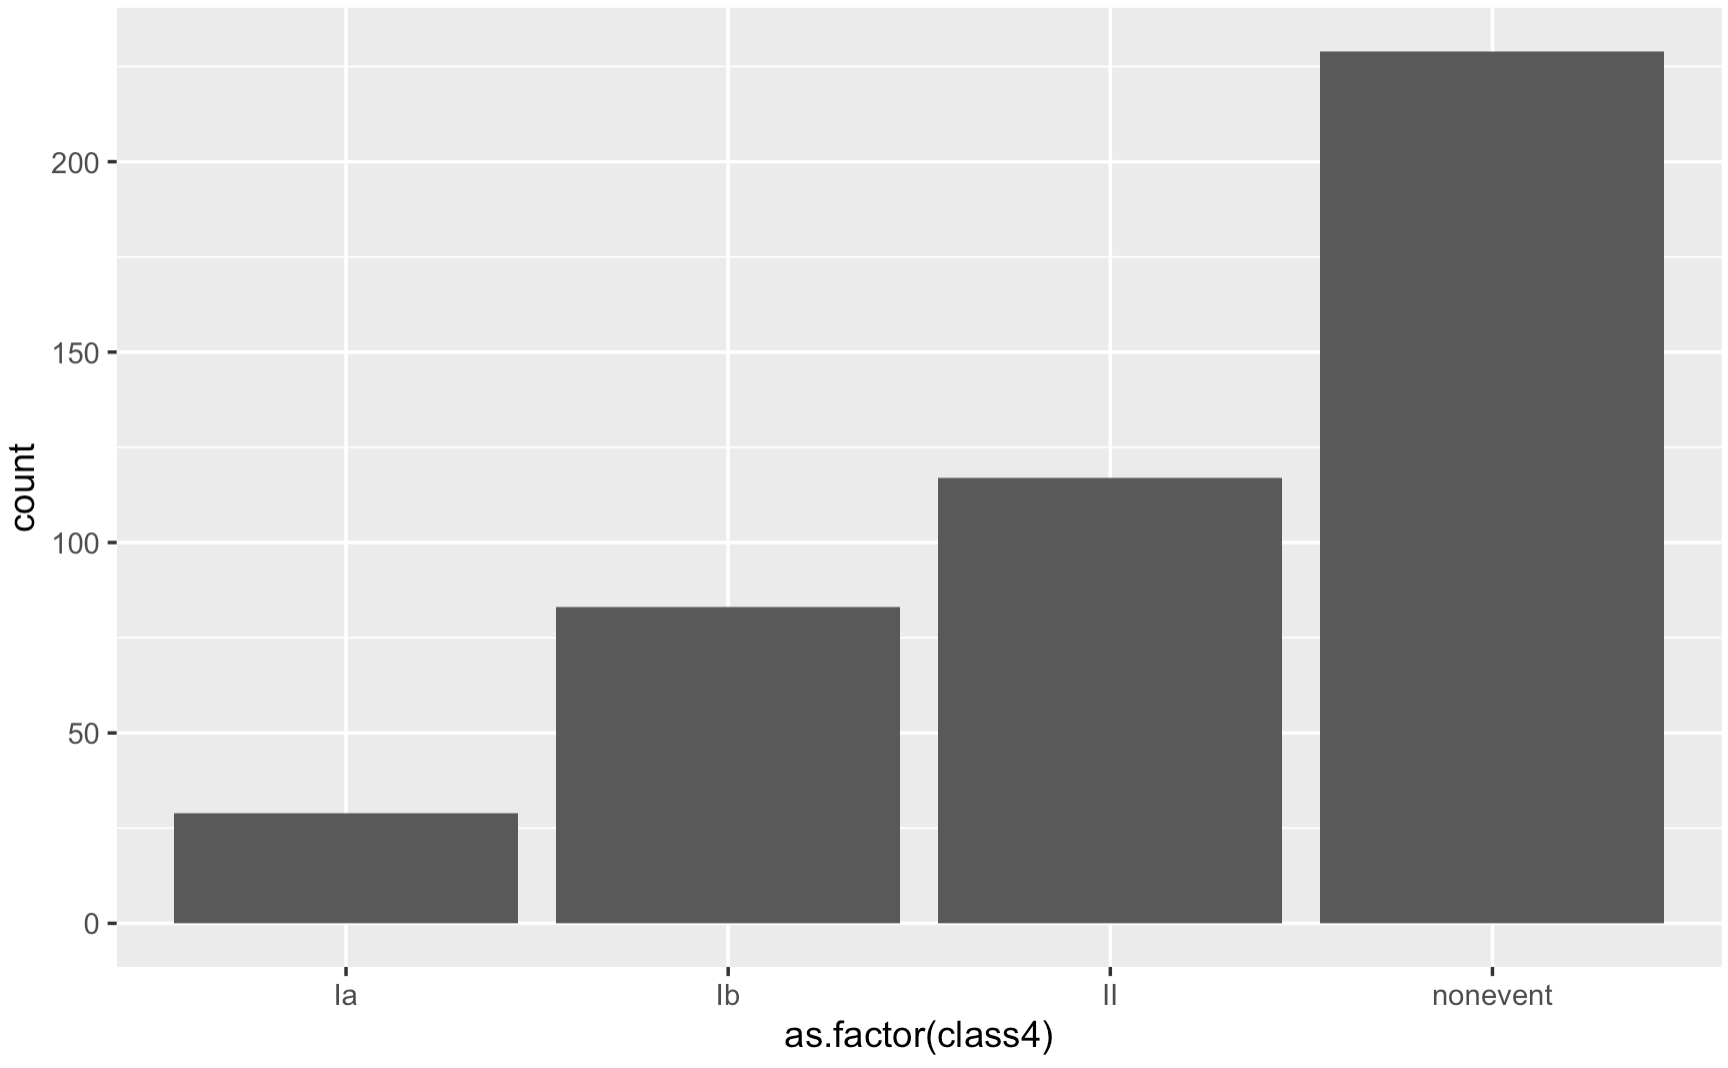
\includegraphics[width=0.65\textwidth]{images/class_distribution.png}
   \caption{Class distribution of the target variable}
   \label{fig:class_distribution}
\end{figure}

% TODO: insert pairplot here and something about it

Both datasets contain 50 variables which are mainly measured at the SMEAR II mast. The variables are further split into their daily means and standard deviations, measured at various times between sunrise and sunset. These consist of relative humidity, carbon monoxide (CO2) concentration, water vapour (H20) concentration, ozone concentration, air temperature, and ultraviolet radiation among others. Some concentrations of the same element are measured at different heights. To understand these height differences better, we provide Figure \ref{fig:height}, where each point indicates the height at which the measurements are taken. These variables are expected to be highly correlated.

\begin{figure}
   \centering
   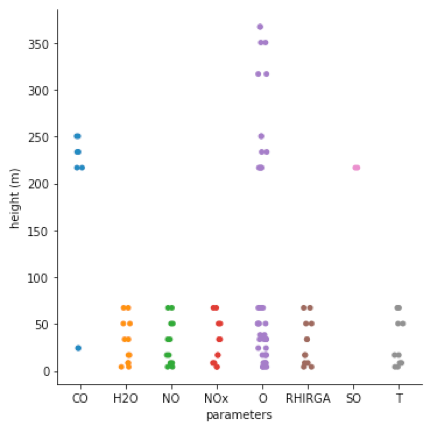
\includegraphics[width=0.5\textwidth]{images/height.png}
   \caption{Heights at which the recordings were taken. Jitter is applied to the points to observe density.}
   \label{fig:height}
\end{figure}

Figure \ref{fig:correlation_matrix} displays a correlation matrix which shows the relationships across the variables. This visualisations only focuses on the mean values of each variable. This restriction is made because while it makes sense to analyze the correlation between the means, the correlation between two standard deviations is unclear. As we stated previously, the measurements of an element at different heights are highly correlated. For example, the correlation coefficient of measurements of H20 at different heights is close to 1.

\begin{figure}[!ht]
   \centering
   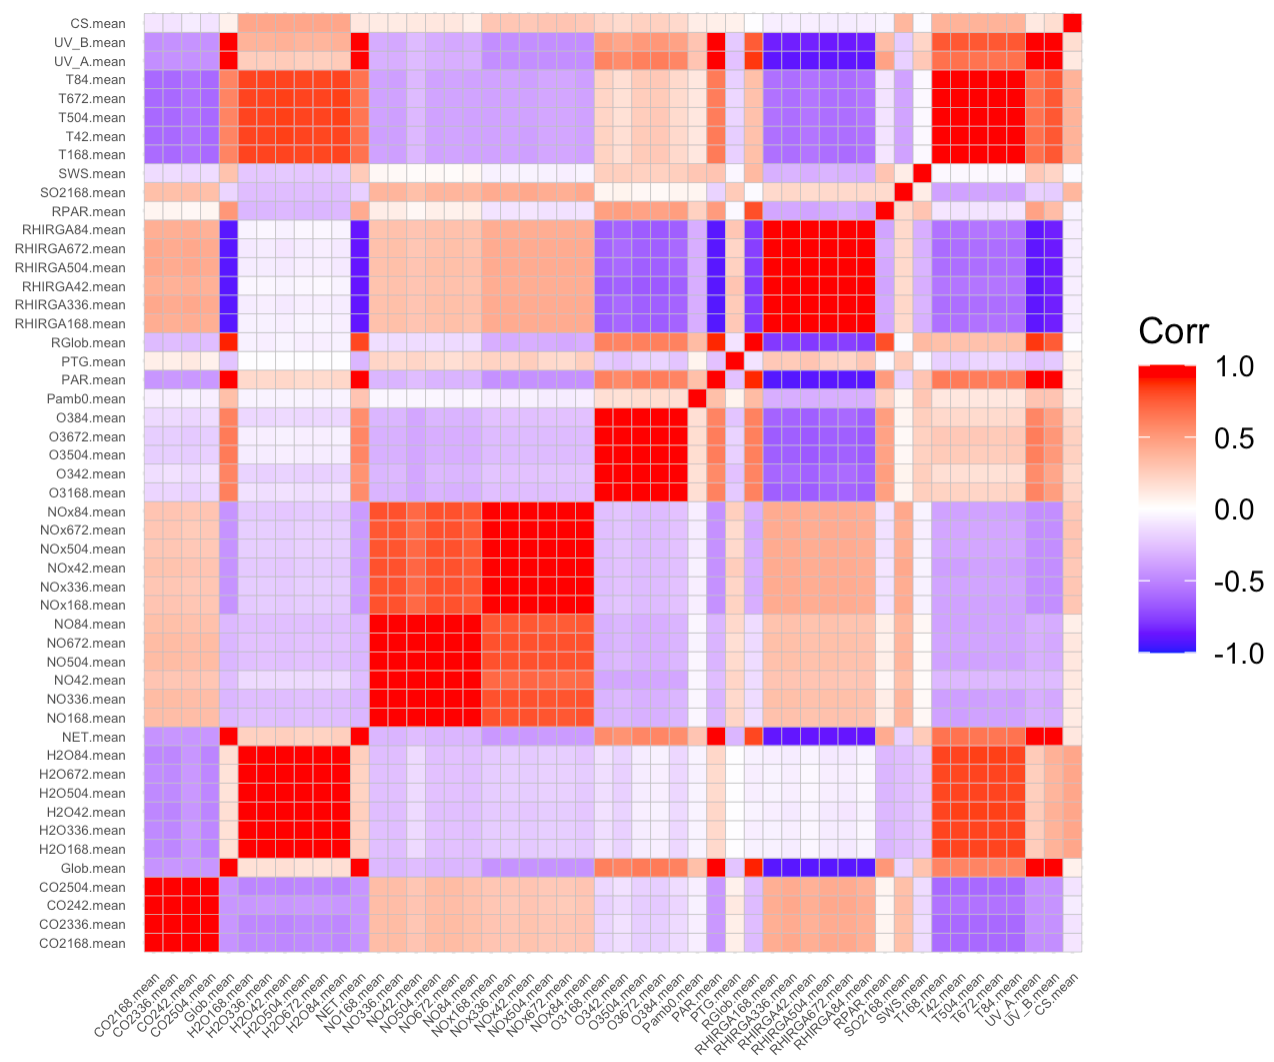
\includegraphics[width=\textwidth]{images/correlation_matrix.png}
   \caption{Correlation matrix between the means of our features}
   \label{fig:correlation_matrix}
\end{figure}

Although not a universal rule, many machine learning algorithms require the variables to be uncorrelated in order to perform optimally. This means that the high correlations between the features must be eliminated before any models are built. The technique used to address this issue is to use dimensionality reduction, which is discussed in the next section.

\section{Dimensionality Reduction}

To address the large set of correlated variables in our data, we use principal component analysis (PCA) as a means of dimensionality reduction. PCA summarizes the correlated variables to a smaller subset which would explain most of their variability \cite{intro_stat_learning}. The main intention is to decrease bias, hence improving generalization accuracy.

Prior to applying PCA, we divided the training dataset into a separate train and test set using stratified sampling, with the test set containing 20\% of the data. The reason for this is so that PCA is fit on the train set only and then applied to the test set in order to avoid overfitting to known data. Any results presented in this section are based on the 80\% of the train set chosen. Furthermore, before any dimensionality reduction is applied, the data is also scaled to mean zero and unit variance.

In PCA, every component explains a part of the variation of the original data. We targeted a 95\% cumulative proportion of variance explained (PVE). Figure \ref{fig:pve} shows the cumulative PVE plotted against the number of principal components. Our target of 95\% cumulative PVE is reached when we have 19 components.

\begin{figure}
   \centering
   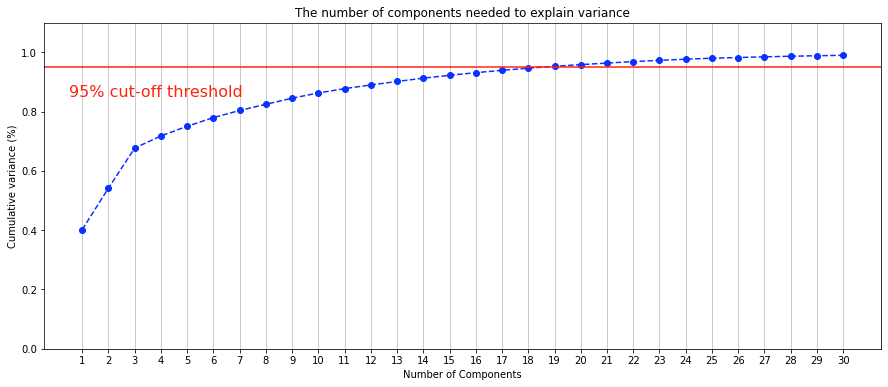
\includegraphics[width=\textwidth]{images/cumulative_pve.png}
   \caption{Cumulative proportion of variance explained against the number of principal components applied on the train set}
   \label{fig:pve}
\end{figure}

Lastly, in order to interpret the PCA results, we show the correlation matrix of the new components against the original features in Figure \ref{fig:pca_correlation_matrix}. One can see, for example, the first component clearly summarizes the means of relative humidity (RHIRGA), while the second component explains the means of H20 and the third one explains NO and NOx. NO and NOx are highly correlated so it makes sense that they form one component.

\begin{figure}[!ht]
   \centering
   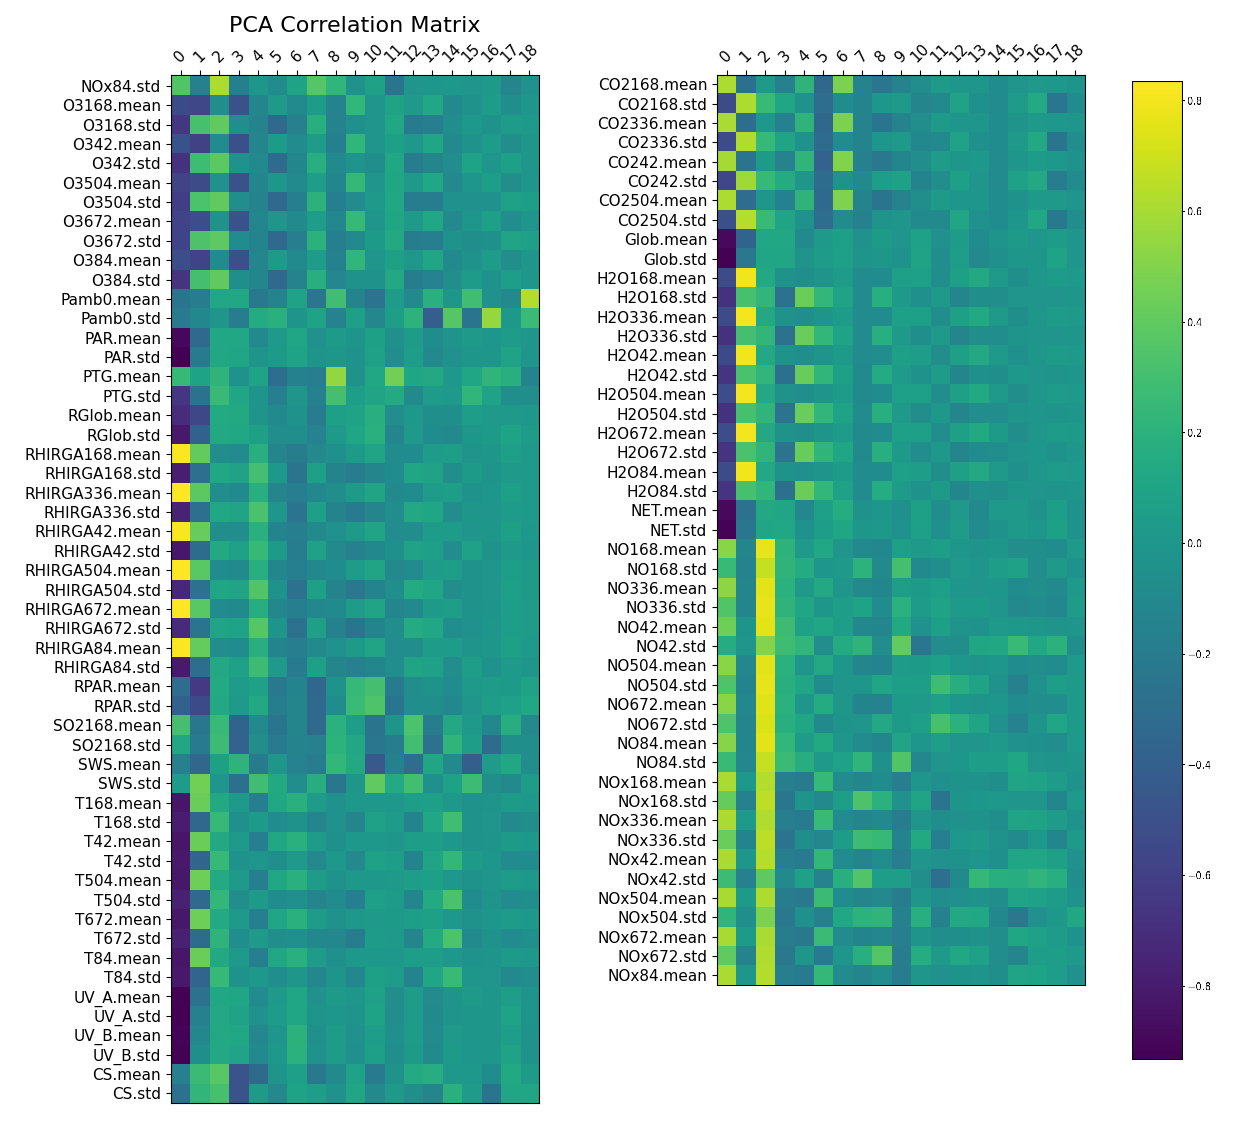
\includegraphics[width=\textwidth]{images/pca_correlation_matrix.png}
   \caption{Correlation matrix between principal components and original features}
   \label{fig:pca_correlation_matrix}
\end{figure}
